\chapter{Introduction}
%\addcontentsline{toc}{chapter}{Introduction}
......
\section{ATLAS Project}\label{sec:ATLAS}
The ATLAS project was created in 2003 by the Group for Automation and Robotics from the Department of Mechanical Engineering at the University of Aveiro \cite{vsantos2010}. The objective of this project is to study and develop advanced sensors and active systems to promote the autonomous control of cars and other platforms. The first projects in the autonomous driving area focused on small scale models in controlled environments for participation in the National Robotics Festival (FNR) and in many other competitions winning some awards for the best performance (subsection \ref{sec:ATLASplatform}). The success and experience gained with these models allowed the evolution of the project for full-scale vehicles, where ATLASCAR (subsection \ref{sec:ATLASCAR}) in 2010 and ATLASCAR2 (subsection \ref{sec:ATLASCAR2}) in 2016 have been developed.

\subsection{ATLAS platforms}\label{sec:ATLASplatform}	
The first developed robot (Figure \ref{fig:modelosatlas1}) was based on an aluminum and wood structure. In this prototype only one camera was installed that pointed to a mirror to allow the complete visualization of the road in which the robot circulated. The traction movement was assured by a mechanical differential coupled to the rear wheels and the steering movement was given by a single front wheel. In order to create a model more similar to an ordinary car, the ATLAS group developed the ATLAS 2000 (Figure \ref{fig:modelosatlas2}) in scale (1:4), with which it managed to win the first autonomous driving competition of the FNR in 2006. After several improvements made in ATLAS 2000, in 2008 a new platform, ATLAS MV (Figure \ref{fig:modelosatlas3}) was created. This robot was designed on a smaller scale (1:5), with the intention of being lighter and faster. On board were installed a new steering system, hydraulic braking and an active perception unit. This robot allowed the conquest of new victories in the autonomus driving competitions.
\begin{figure}[!h]
	\centering
		\begin{minipage}[t]{0.32\textwidth}
			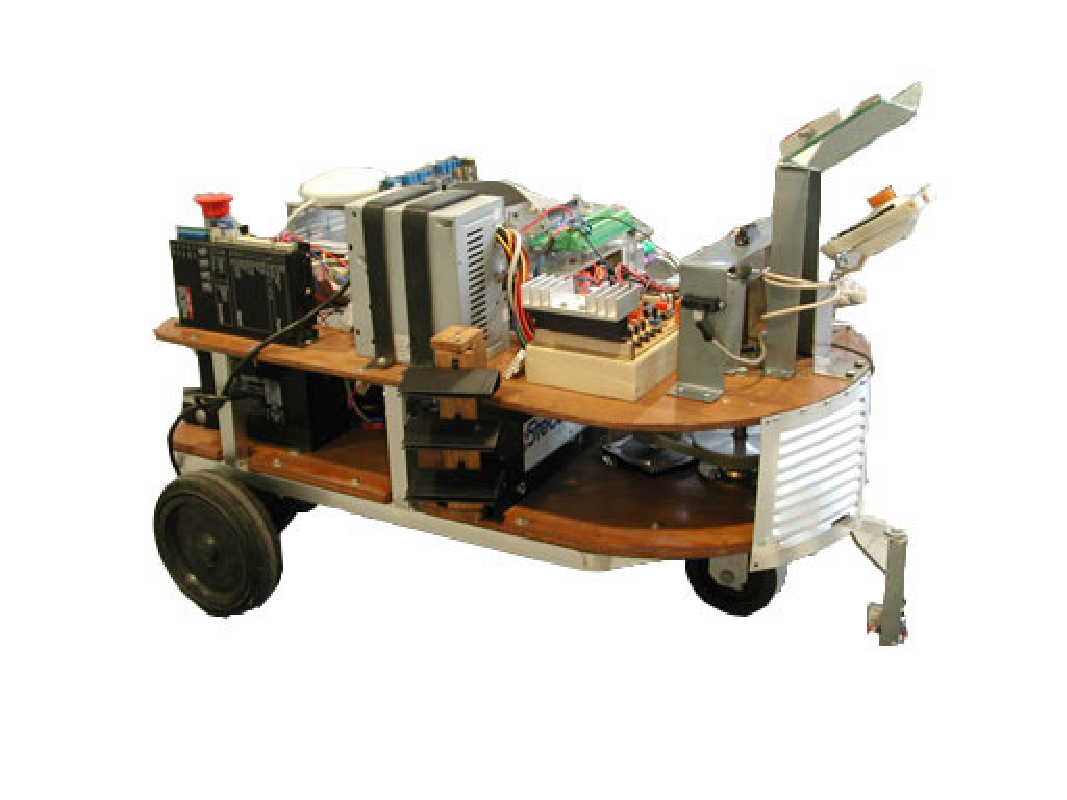
\includegraphics[width=\textwidth]{../figure/modelosatlas1.pdf}
			\subcaption{First ATLAS prototype.}
			\label{fig:modelosatlas1}
		\end{minipage}
		\begin{minipage}[t]{0.32\textwidth}
			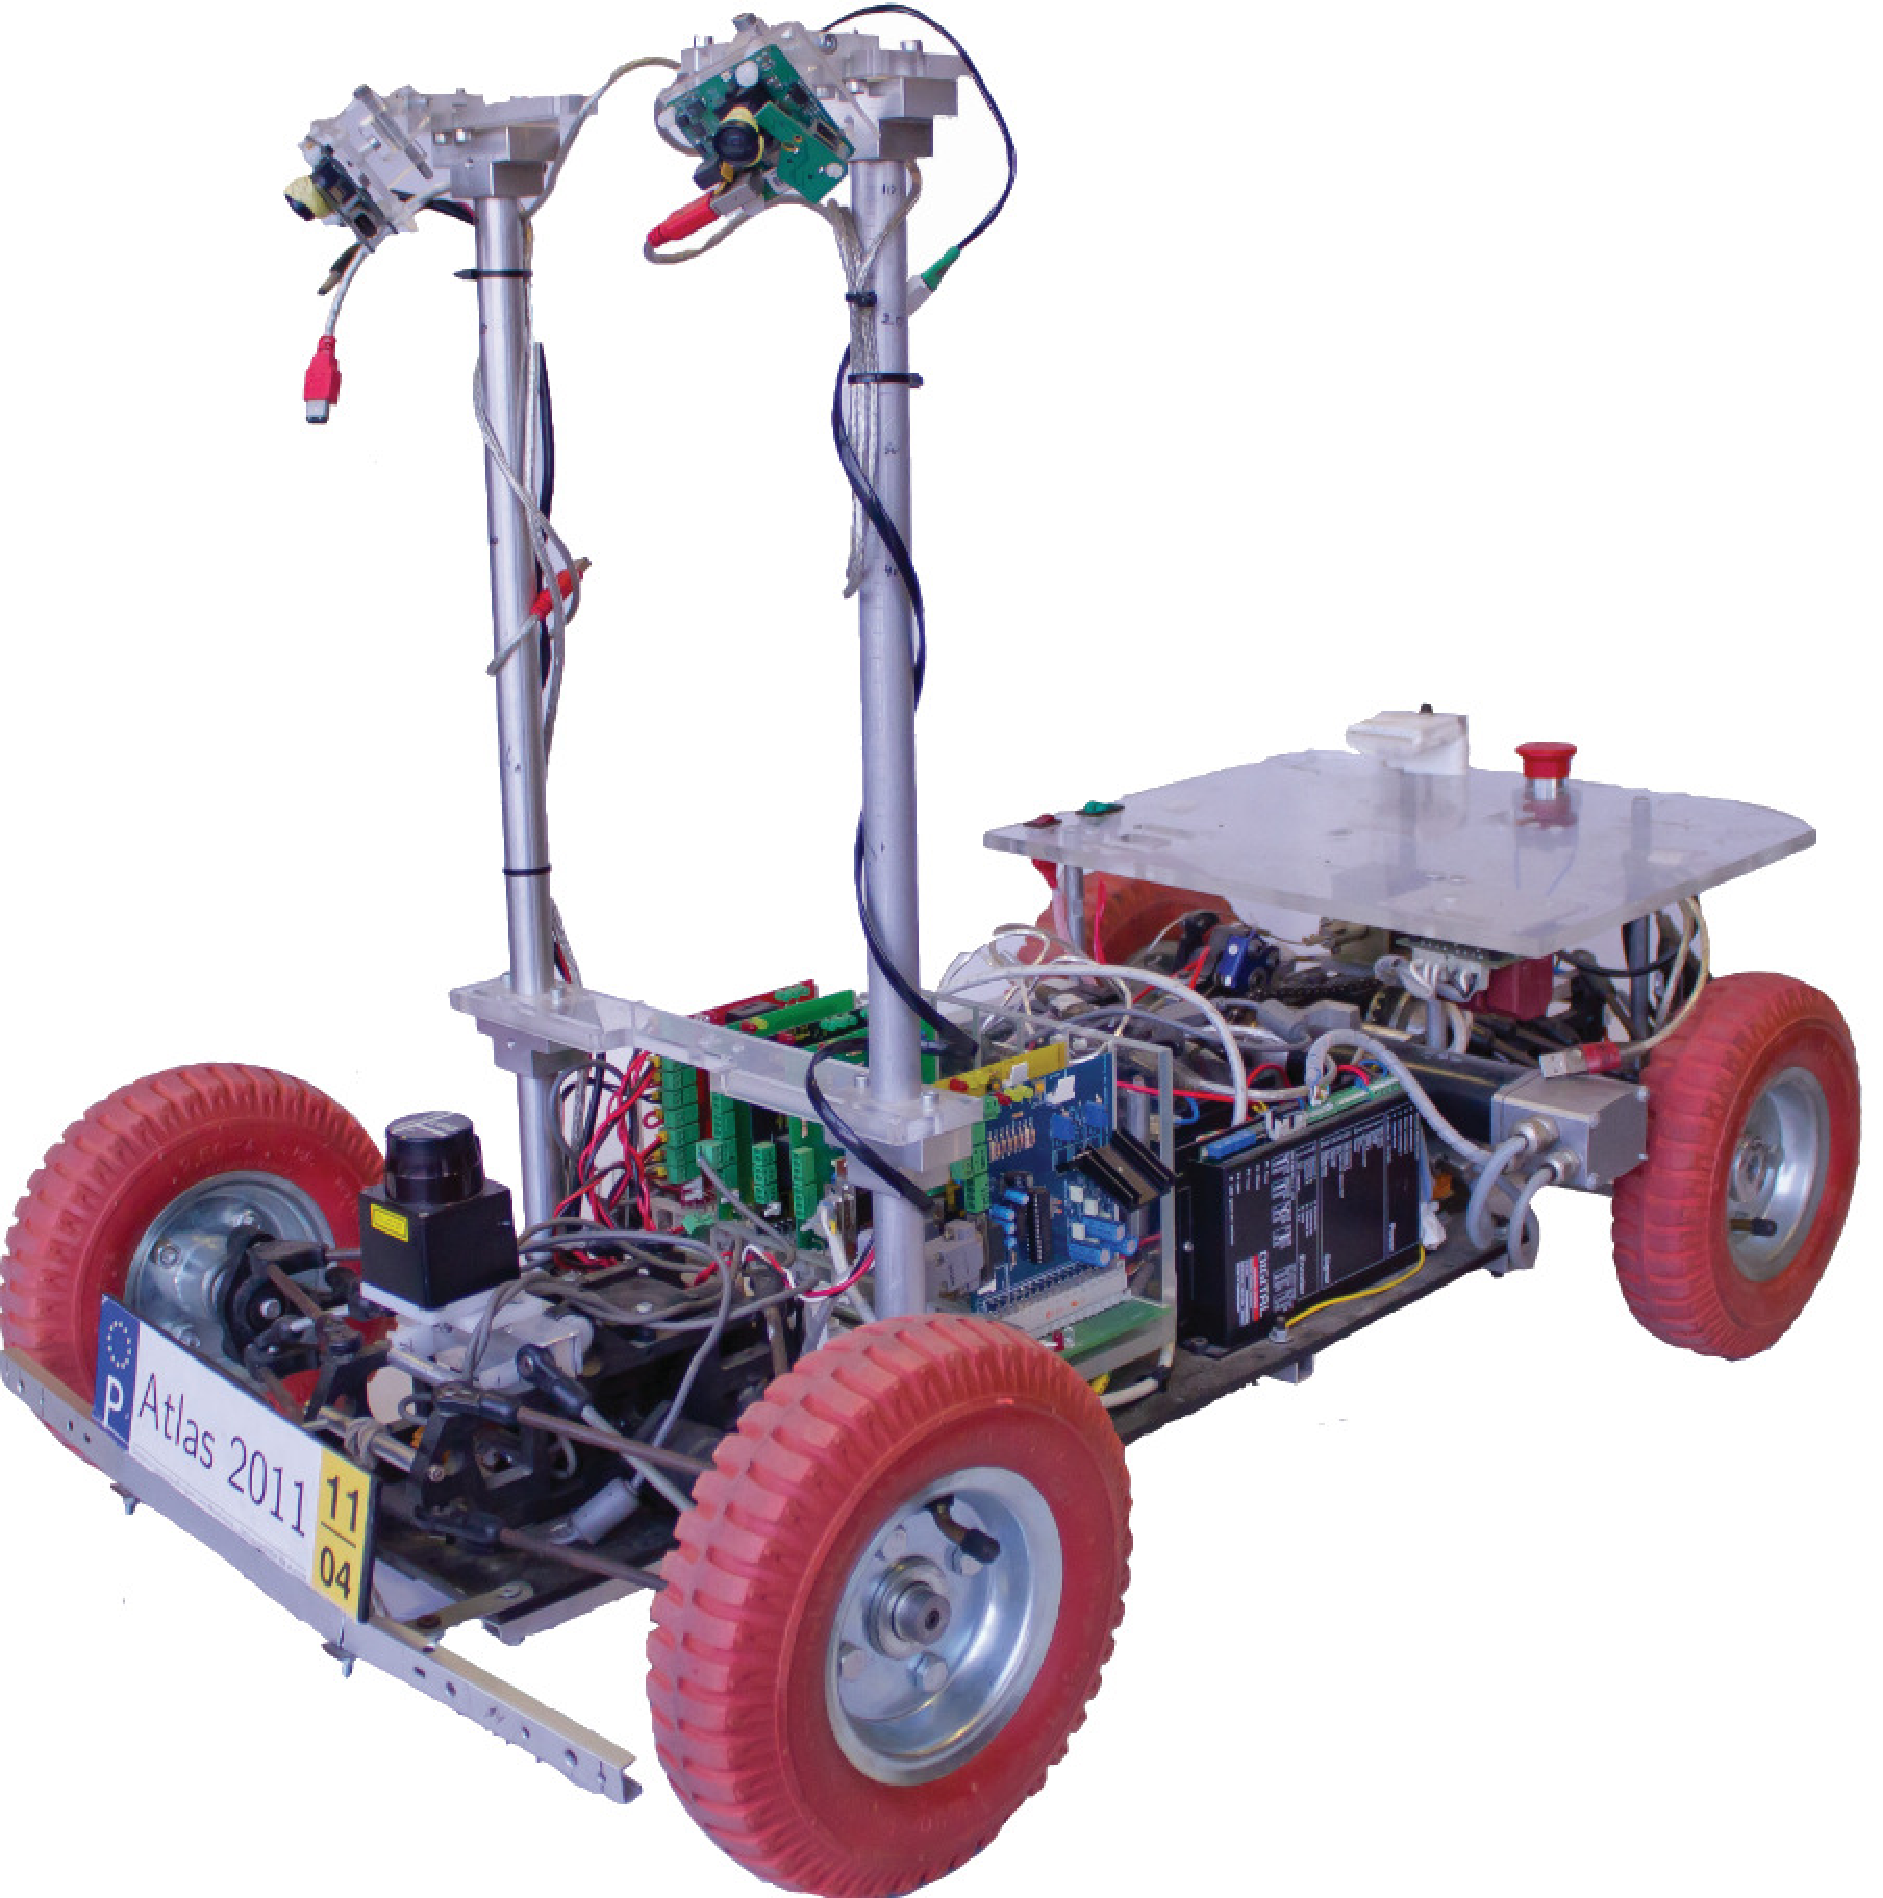
\includegraphics[width=\textwidth]{../figure/modelosatlas2.pdf}
			\subcaption{ATLAS 2000.}
			\label{fig:modelosatlas2}
		\end{minipage}
		\begin{minipage}[t]{0.32\textwidth}
			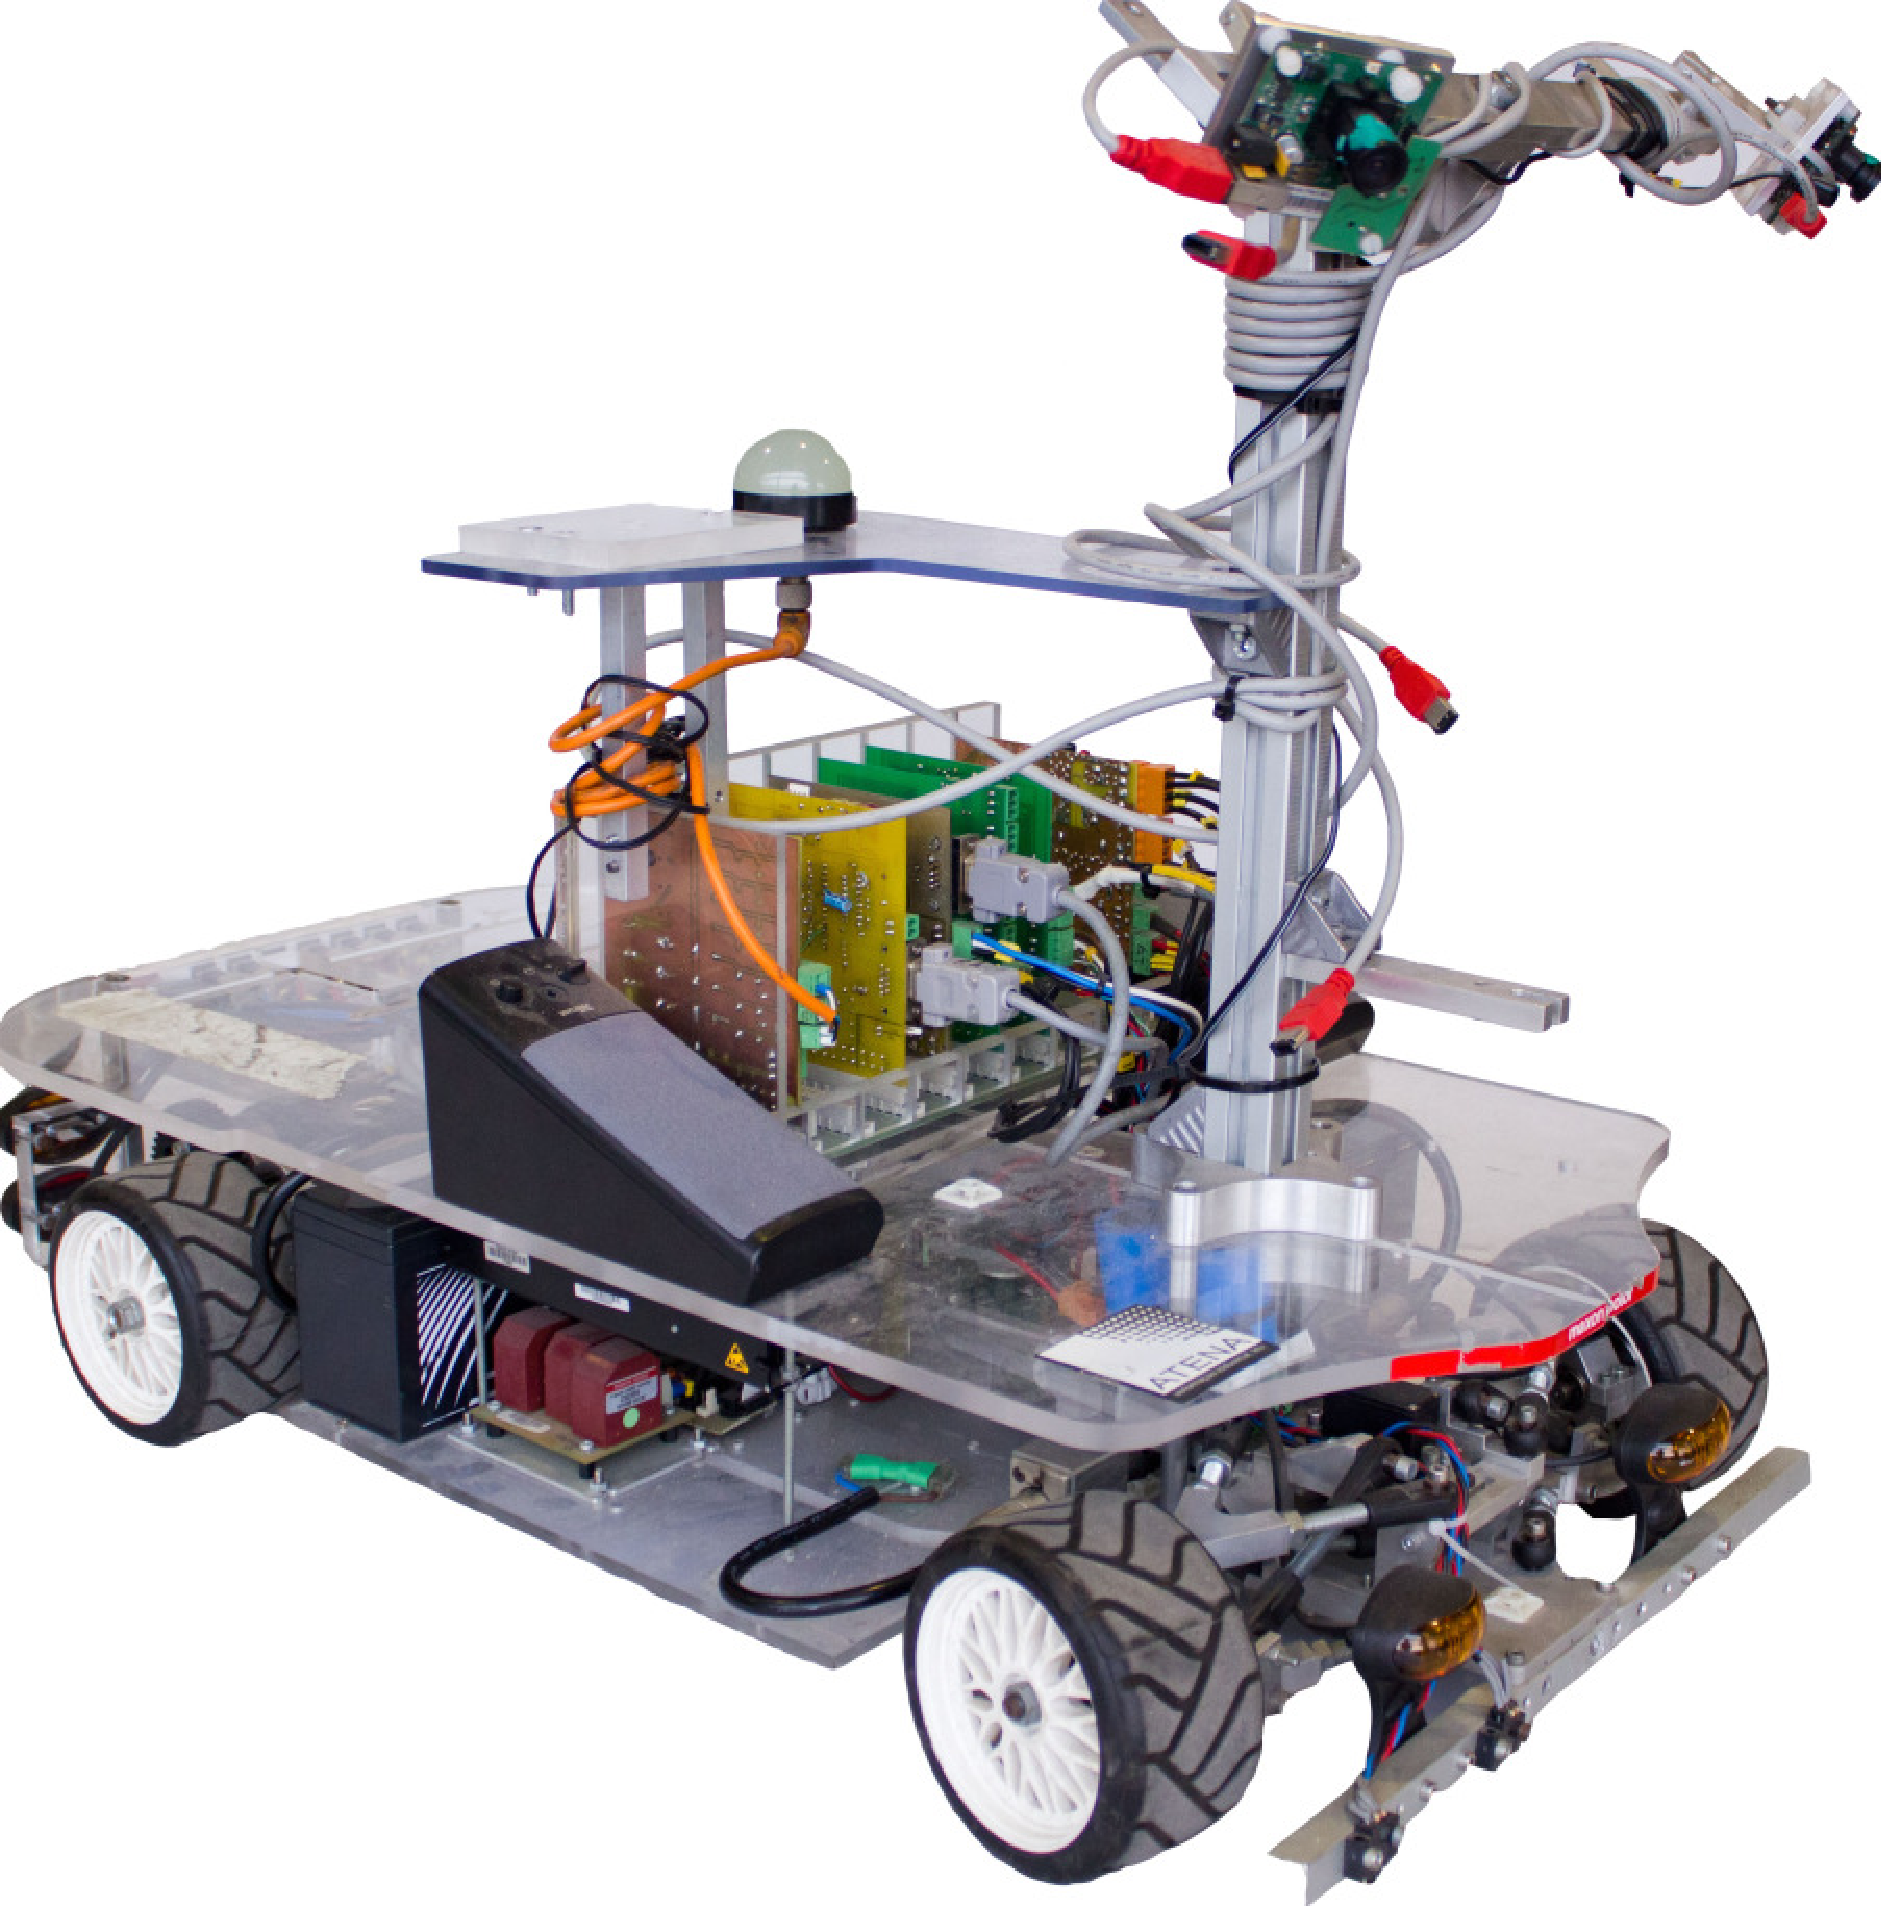
\includegraphics[width=\textwidth]{../figure/modelosatlas3.pdf}
			\subcaption{ATLAS MV.}
			\label{fig:modelosatlas3}
		\end{minipage}
		\caption{Some of the ATLAS project small scale platforms (adapted from \cite{Pereira2012}).}
		\label{fig:modelosatlas}
\end{figure}

\subsection{ATLASCAR}\label{sec:ATLASCAR}
Driven by the positive results achieved with scale models and years of navigation experience in controlled environments, in 2010 the Group of Automation and Robotics decided to invest in a large-scale project, ATLASCAR (Figure \ref{fig:atlascar1}). The vehicle used for this project was a Ford Escort Station Wagon of 1998 powered by a gasoline internal combustion engine, in which several sensors, processing units and actuators were installed. On-board sensors processed data collected from the vehicle and its surroundings, with different LIDARs for obstacle detection and environmental reconstruction, pedestrian detection cameras and a Global Navigation Satellite System (GNSS) for location and route planning. After passing through the processing units, these data were sent to the actuators that allowed the movement and execution of the maneuvers in a completely autonomous way on the part of the vehicle. To power all the equipment, a Uninterruptible Power Supply (UPS) was used, loaded from an auxiliary alternator. During this project, many works were developed in the Laboratory for Automation and Robotics, many of which produced master thesis. For example, in 2014 Cabral de Azevedo \cite{Azevedo2014} developed a module to detect pedestrians using sensory fusion of LIDAR and vision data while in 2016 Vieira da Silva \cite{Silva2016} created a multisensory calibration module that was exported to subsequent projects.
\begin{figure}[!h]
	\centering
	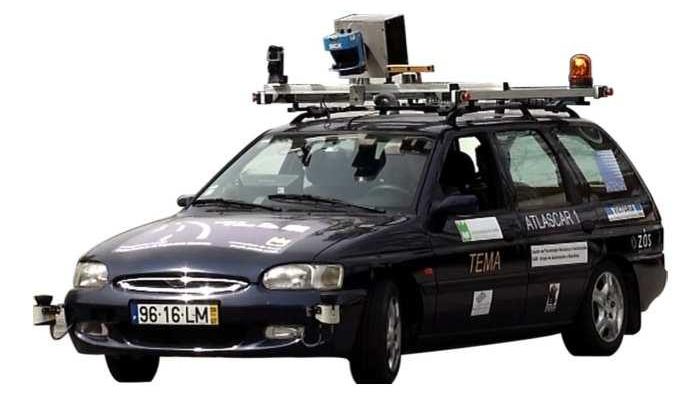
\includegraphics[width=\textwidth]{../figure/atlascar1.jpg}
	\caption{The car used in ATLASCAR, based on Ford Escort Station Wagon of 1998 (adapted from \cite{Pereira2012}).}
	\label{fig:atlascar1}
\end{figure}

\subsection{ATLASCAR2}\label{sec:ATLASCAR2}
Given the different limits, to continue the project, in 2016, a new vehicle was acquired: ATLASCAR2 (Figure \ref{fig:atlascar2}). This time it was chosen as a platform
an electric car, a Mitsubishi iMiEV, with an autonomy range of \SI{100}{km}. The fact that the vehicle is electric allows to use the energy stored in the batteries, making it easier to power the sensors installed. In fact, despite the short time of existence, 3 LIDARs, a camera, inclinometry sensors and a GNSS unit are already installed on the ATLASCAR2. Many of these sensors were transferred from ATLASCAR to this project during the work of Madureira Correia \cite{Madureira2017} in 2017, where a module for detecting free space around the car was also developed while in 2018 Ricardo Silva \cite{Ricardo:Thesis:2018} created a local navigation module for driver assistance in the immediate decision making, identifing a solution based on a multiple hypothesis approach.
\begin{figure}[!h]
	\centering
	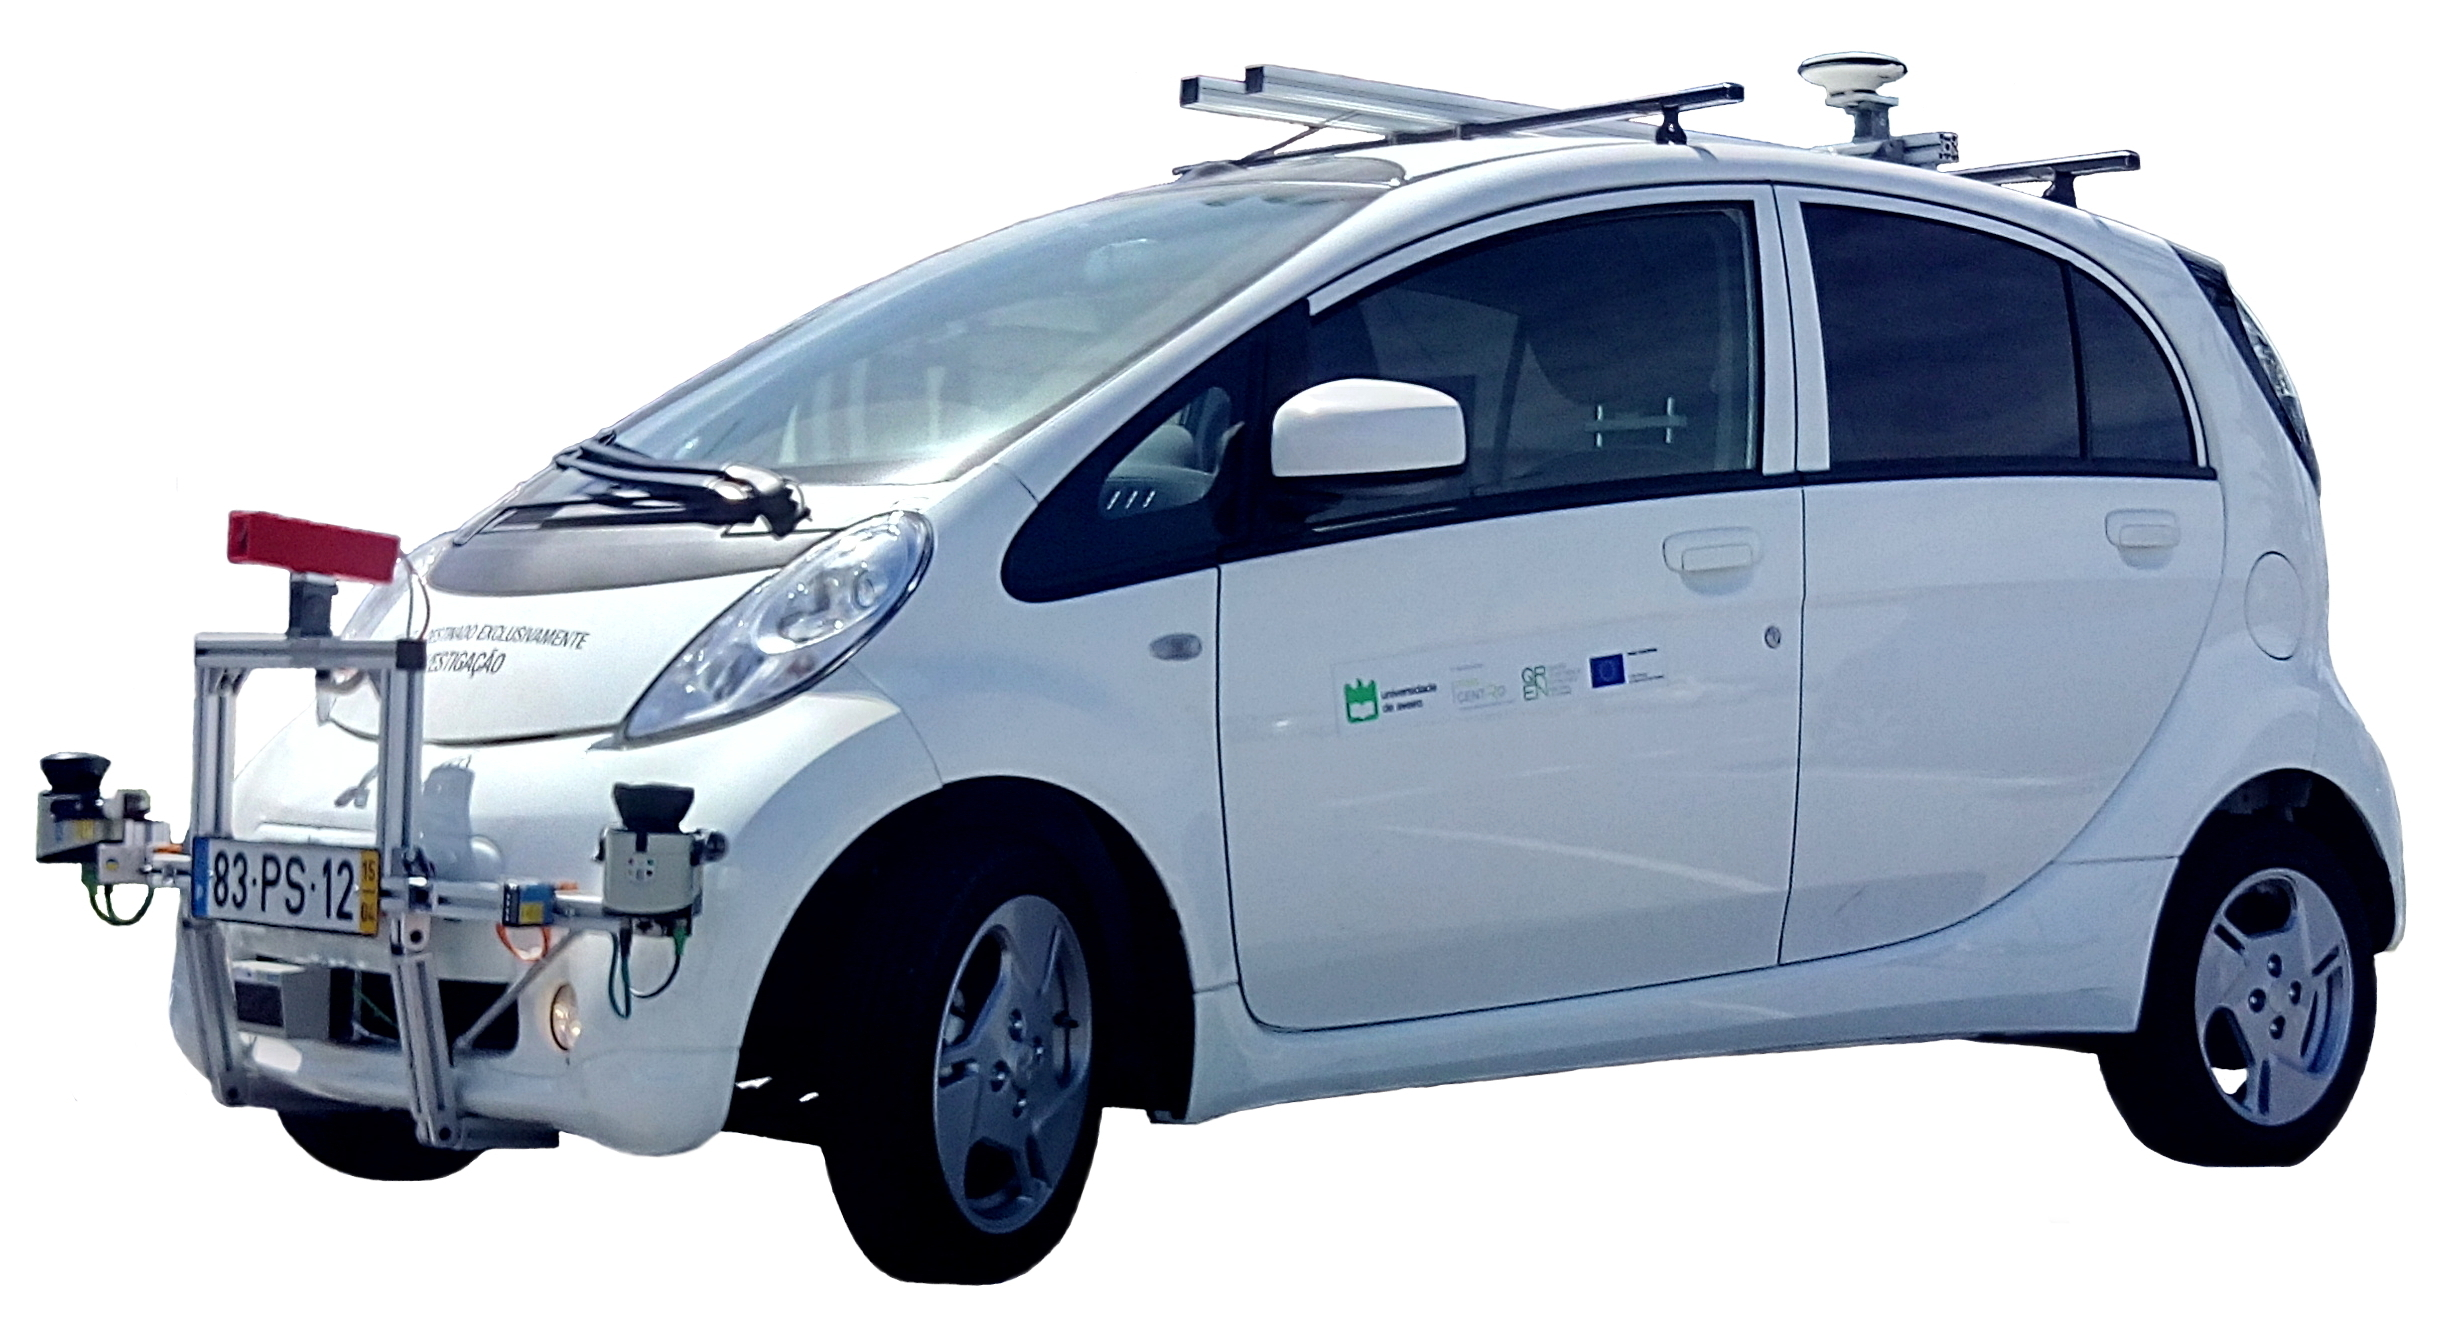
\includegraphics[width=\textwidth]{../figure/atlascar2.jpg}
	\caption{The vehicle used in ATLASCAR2, based on an electric car, a Mitsubishi iMiEV of 2015 (adapted from \cite{Ricardo:Thesis:2018}).}
	\label{fig:atlascar2}
\end{figure}

\section{Autonomous Cars}
The modern automobile companies keep coming up with newer autonomous features in their recent models. Technological advancements seen every day in areas like information technology, communication, data analysis and storage etc. is not exclusive to these areas alone. The realm of autonomous cars is also progressing at a rapid rate these days \cite{Bimbraw2015}. Google's development of self-driving technology began in January 2009. The initial objective of the project was to develop a car able to navigate on highways with minimal human intervention. In December 2016, the unit was renamed Waymo; this name derived from its mission, "a new way forward in mobility". Waymo moved to further test its cars on public roads after becoming its own subsidiary.
\begin{figure}[!h]
	\centering
	\begin{minipage}[t]{0.65\textwidth}
		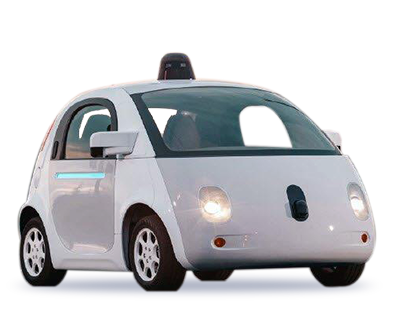
\includegraphics[width=\textwidth]{../figure/veiculos0.png}
		\subcaption{Google's Firefly self-driving prototype in 2015 (adapted from \cite{waymoh}).}
		\label{fig:veiculos0}
	\end{minipage}
	\begin{minipage}[t]{0.65\textwidth}
		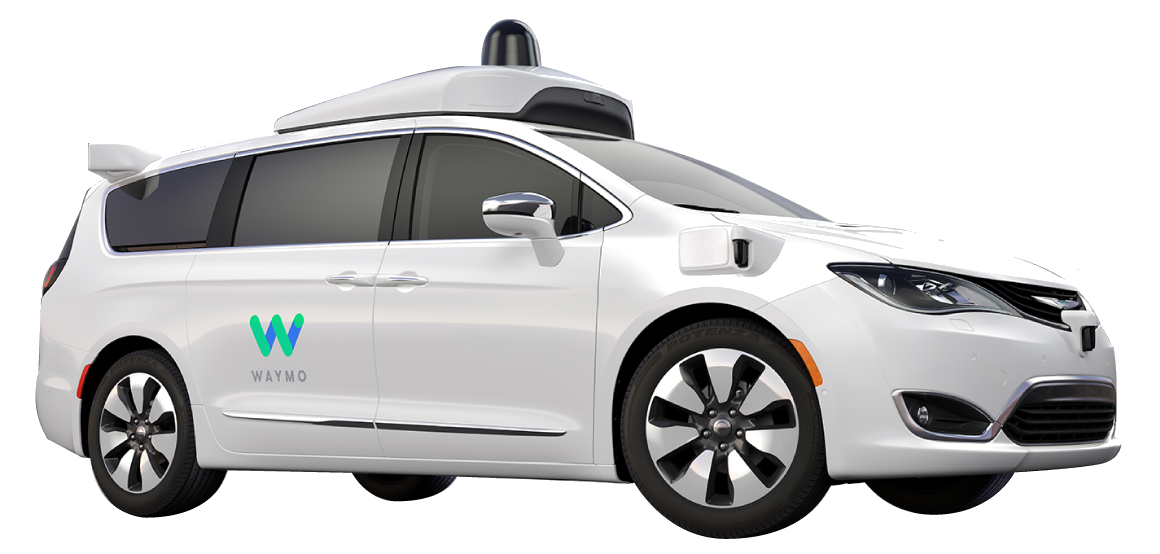
\includegraphics[width=\textwidth]{../figure/veiculos1.png}
		\subcaption{Waymo Chrysler Pacifica Hybrid self-driving prototype in 2017 (adapted from \cite{waymoh}).}
		\label{fig:veiculos1}
	\end{minipage}
	\caption{Some of the Waymo/Google prototypes tested across multiple locations in the Unided States in recent years.}
	\label{fig:waymo}
\end{figure}

Waymo uses LIDAR which sends out millions of laser beams per second to build up a detailed picture of the world all 360 degrees around it. It also uses radar to detect how far away objects are and their speed and high-resolution cameras detect visual information like whether a traffic signal is red or green. It then combines all that data to understand the world around it and predict what those things might do next. It can do that for things up to three football fields away. Based on all this information, Waymo's software determines the exact trajectory, speed, lane and steering maneuvers needed to progress along this route safely \cite{waymoh} \cite{waymot}.
With the advances in autonomous technology, VIAC or VisLab Intercontinental Autonomous Challenge was one of the major competitions which led to improvements in the testing and analysis of autonomous vehicles and robotics. It was a 13,000 kilometers trip, nearly three months from Parma, Italy to Shanghai, China from July 20, 2010 to October 28, 2010. It involved four autonomous vehicles with negligible human intervention and high level of autonomy \cite{Broggi2010}.
\begin{figure}[!h]
	\centering
	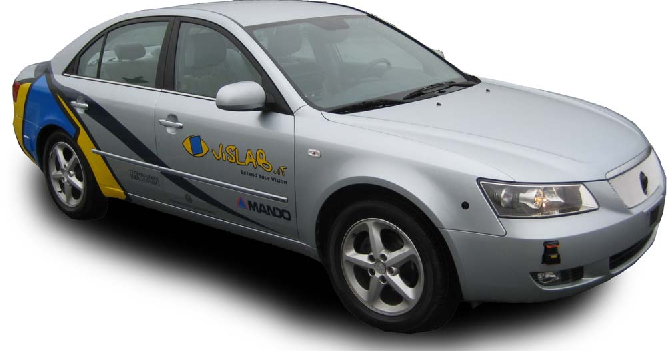
\includegraphics[width=0.65\textwidth]{../figure/veiculos4.png}
	\caption{BRAiVE prototype developted by VisLab, based on a Hyundai Sonata (adapted from \cite{Broggi2013}).}
	\label{fig:veiculos4}
\end{figure}
\section{Context of the Problem and Motivation}
\section{Proposed Approach}
\section{Thesis Outline and Contributions}